\documentclass{beamer}
\usetheme{CambridgeUS}
\usepackage[utf8]{inputenc}
\usepackage[russian]{babel}
\usepackage{listings}
\usepackage{xcolor}
\usepackage{hyperref}
\usepackage{graphicx}
\setbeamercolor{item}{fg=red}

\lstset{
	basicstyle=\bfseries\ttfamily,
	keywordstyle=\bfseries\color{blue},
	commentstyle=\bfseries\color{gray},
	stringstyle=\bfseries\color{red},
	tabsize=2,
	showstringspaces=false,
	breaklines=true,
	captionpos=b,
	frame=none,
	numbers=none,
}

\hypersetup{
	colorlinks=true,
	linkcolor=black,
	urlcolor=blue
}

\title{Учебный компилятор}
\author[Балышев А.М.]{Автор: Балышев А.М. \\ Руководитель: Косарев Д.С.}

\begin{document}
	\begin{frame}[plain]
		\maketitle
	\end{frame}
	
	\begin{frame}
	\frametitle{Язык и платформа}
	\begin{itemize}
			\item Язык — OCaml
			\item Хостинг кода — GitHub
			\item CI/CD — GitHub Actions
		\end{itemize}
	\end{frame}
	
	\begin{frame}
		\frametitle{Цель и задачи}
		\textbf{Цель:} \\
		Создание AOT-компилятора вымышленного императивного языка, способного компилировать относительно несложные программы
		\textbf{Задачи:}\\
		\begin{itemize}
			\item Реализация фронтенда
			\begin{itemize}
				\item Лексический разбор
				\item Синтаксический разбор
				\item Семантический разбор
			\end{itemize}
			\item Реализация бэкенда
			\begin{itemize}
				\item Порождение RISC-V Assembly
			\end{itemize}
		\end{itemize}
	\end{frame}
	
	\begin{frame}
		\frametitle{О компилируемом языке}
		\begin{itemize}
			\item Поддержка базовых императивных конструкций
			\begin{itemize}
				\item Объявления и присваивания
				\item Циклы
				\item Ветвления
				\item Описание и вызов процедур
			\end{itemize}
			\item Поддержка типов и областей видимости
		\end{itemize}
	\end{frame}
	
	\begin{frame}[fragile]
		\frametitle{Пример}
	\begin{lstlisting}[language=BASH] 
var a b j;

a := 0;
b := 1;
j := 0;

while j < 8 do
	print a;
	b := a + b;
	a := b - a;
	j := j + 1;
done
	\end{lstlisting}
	\end{frame}

	\begin{frame}
		\frametitle{О процессе компиляции}
			\begin{itemize}
			\item Каждый этап обрабатывается отдельной функцией
			\item Функция принимает некоторое представление программы и возвращает новое представление, снабженное дополнительной информацией
			\item Компиляция осуществляется путём последовательного применения этих функций
			\end{itemize}
	\end{frame}
	
	\begin{frame}{Этапы построения исполняемого модуля}
		\begin{center}
			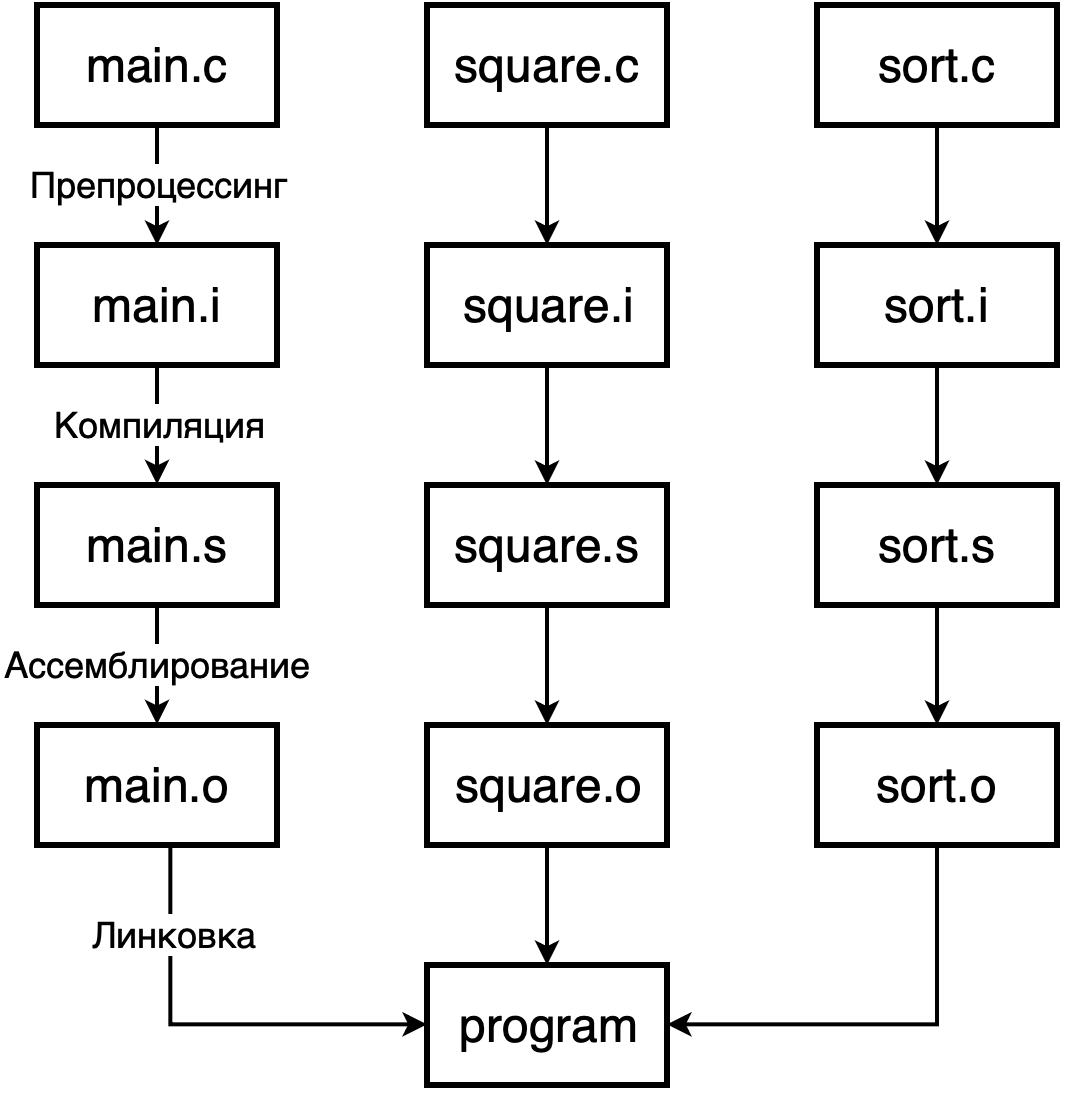
\includegraphics[width=0.5\linewidth]{stages.jpg}
		\end{center}
	\end{frame}
	
	\begin{frame}{Этапы компиляции}
		\begin{center}
			\hspace{1.5cm}
			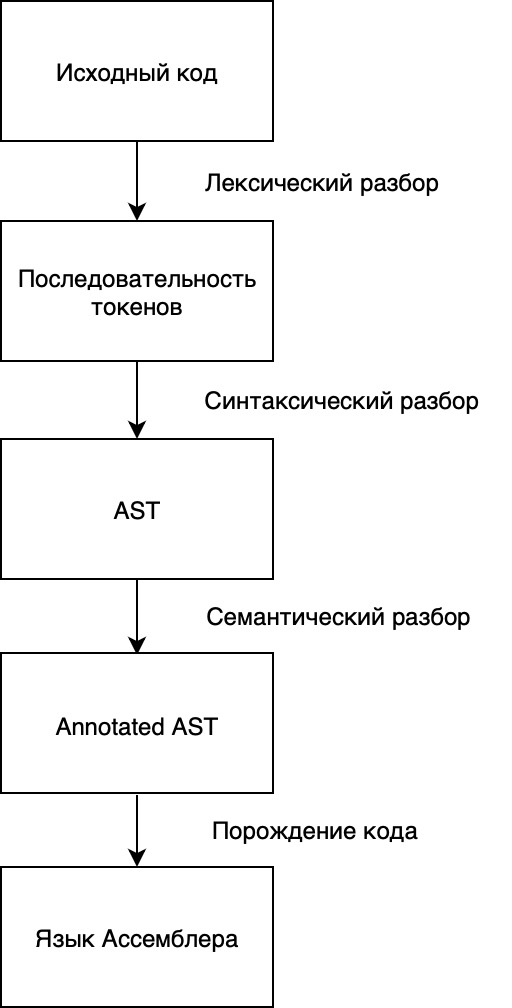
\includegraphics[width=0.3\linewidth]{compilation.jpg}
		\end{center}
	\end{frame}

	\begin{frame}[fragile]
		\frametitle{Лексический разбор}
			Задачи:
			\begin{itemize}
				\item Преобразовать исходный код в последовательность токенов
				\item Выявить лексические ошибки
			\end{itemize}
			Сигнатура функции:
			\begin{lstlisting}[language=ML] 
	val tokenize : string -> token list
			\end{lstlisting}
			В качестве токенов могут выступать:
			\begin{itemize}
				\item Ключевые слова
				\begin{itemize}
					\item \lstinline[language=BASH]|while, do, done, if, then, else, fi ...|
				\end{itemize}
				\item Литералы
				\begin{itemize}
					\item \lstinline[language=ML]|Int(123), True, False, String("hello world")|
				\end{itemize}
				\item Унарные и бинарные операторы и скобки
				\item Идентификаторы переменных и функций
			\end{itemize}
	\end{frame}

	\begin{frame}[fragile]
		\frametitle{Синтаксический разбор}
		Задачи:
		\begin{itemize}
			\item Преобразовать последовательность токенов в AST
			\item Выявить синтаксические ошибки
		\end{itemize}
		Сигнатура функции:	
		\begin{lstlisting}[language=ML] 
	val construct_ast : token list -> program
		\end{lstlisting}
		\end{frame}

	\begin{frame}[fragile]
		\frametitle{AST}
		\begin{lstlisting}[language=ML] 
type program = statement list

type statement =
| Assignment of string * expression
| While of expression * program
| Ite of expression * program * program
| ...

type expression =
| Var of string
| Int of int
| BinOp of operation * expression * expression
| ...
		\end{lstlisting}
	\end{frame}
	
		\begin{frame}[fragile]
			\frametitle{Семантический разбор}
			Задачи:
			\begin{itemize}
				\item Дополнить AST информацией о типах и областях видимости
				\item Выявить семантические ошибки
			\end{itemize}
			Сигнатура функции:
			\begin{lstlisting}[language=ML] 
		val annotate_ast : program -> typed_program
			\end{lstlisting}
			Поддерживаемые на данный момент типы:
			\begin{itemize}
				\item Int
				\item Bool
				\item String
			\end{itemize}
		\end{frame}

	\begin{frame}[fragile]
		\frametitle{Annotated AST}
		\begin{lstlisting}[basicstyle=\footnotesize\ttfamily, language=ML]
type typed_program = (typed_statement * scope) list

type typed_statement =
| Assignment of string * typed_expression
| While of typed_expression * typed_program
| Ite of typed_expression * typed_program * typed_program
| ...

type typed_expression =
| Type_Int of ...
| Type_Bool of ...
| Type_Str of ...
		\end{lstlisting}
	\end{frame}

	\begin{frame}[fragile]
		\frametitle{Порождение кода}
		Задача:
		\begin{itemize}
			\item Генерация языка Ассемблера по AST
		\end{itemize}
		\\
		Сигнатура функции:
		\begin{lstlisting}[language=ML] 
	val generate_assembly : annotated_ast -> string
		\end{lstlisting}

		\begin{itemize}
			\item Порождение кода реализовано для RISC-V 64-bit
			\item Локальные переменные размещаются в стеке
			\item ASCIIZ-строки — в куче
		\end{itemize}
	\end{frame}

	\begin{frame}
		\frametitle{Дальнейшие этапы}
		\begin{itemize}
			\item Ассемблирование
			\begin{itemize}
				\item Например, с помощью \lstinline|riscv64-unknown-elf-as|
				\item Результат — объектный модуль
			\end{itemize}
			\item Линковка
				\begin{itemize}
					\item Например, с помощью \lstinline|riscv64-unknown-elf-ld|
					\item Результат — исполняемый файл
				\end{itemize}
			\item Исполнение
			\begin{itemize}
				\item Или нативно, если архитектура соответствующая
				\item Или с помощью эмулятора, например \lstinline|qemu|
			\end{itemize}
		\end{itemize}
	\end{frame}

	\begin{frame}
		\frametitle{О проблемах и решениях}
		\begin{itemize}
			\item Восстановление \lstinline|sp| при выходе из \lstinline|scope|'а
			\begin{itemize}
				\item Можно передавать в \lstinline|scope| и возвращать из него количество переменных на стеке
			\end{itemize}
			\item Затенение переменных и функций
			\begin{itemize}		
				\item Можно хранить и искать содержимое \lstinline|scope| в порядке объявления
			\end{itemize}
			\item Метки не должны повторяться
			\begin{itemize}
				\item Можно генерировать их случайно
			\end{itemize}
		\end{itemize}
	\end{frame}

	\begin{frame}
		\frametitle{Заключение}
			Использовавшиеся инструменты:
			\begin{itemize}
				\item \lstinline|ppx_expect|, \lstinline|ppx_deriving|
				\item \lstinline|ocamlformat|
				\item \lstinline|riscv64-unknown-elf-as|
				\item \lstinline|riscv64-unknown-elf-ld|
				\item \lstinline|qemu-riscv64|
				\item \lstinline|spike|
			\end{itemize}
			Ссылка на репозиторий: \url{https://github.com/psiblvdegod/compiler}
	\end{frame}
\end{document}
